\chapter{Discrete Dynamical Systems}
They are systems where the evolution is performed using discrete steps, in which the variables describing the state of the system are updated.

\section{Recurrence relations (Difference equations)}
Relations that tell you how from the current state of the discrete systems you obtain the next state of the systems, that is how from the original values the go to the new ones.
\par In this schema we will consider a generic system that is considered as a \textbf{population}(birth/death of individuals). Even the simplest form of interaction between individuals can lead to the emergence of \textbf{complex behaviors} (chaotic behavior) in the population. 

\section{Linear Birth Model}
The linear birth model is the simplest model describing a recurrence relation.
\par Given a population, each individual is \textbf{indistinguishable} from each other. We denote with \texttt{N(t)} the \textbf{density of some population} at a time \texttt{t}, that is the variable that describe the number of individuals that are part of the population at time \texttt{t}.
\par Given this description we want to predict what will happen to the density of the same population at a future time $t^{'} = t + \Delta{t}$ assuming that:

\begin{itemize}
    \item all individuals are indistinguishable from each other.
    
    \item there is enough food and space for every individual.
    
    \item each individual has $\lambda$ children every $\sigma$ time units.

    \item there is no death occurring in the interval $ [t, t + \Delta{t} )$.

    \item children do not start reproducing in the interval $ [t, t + \Delta{t} )$.
\end{itemize}

\begin{figure}[h]
    \centering
    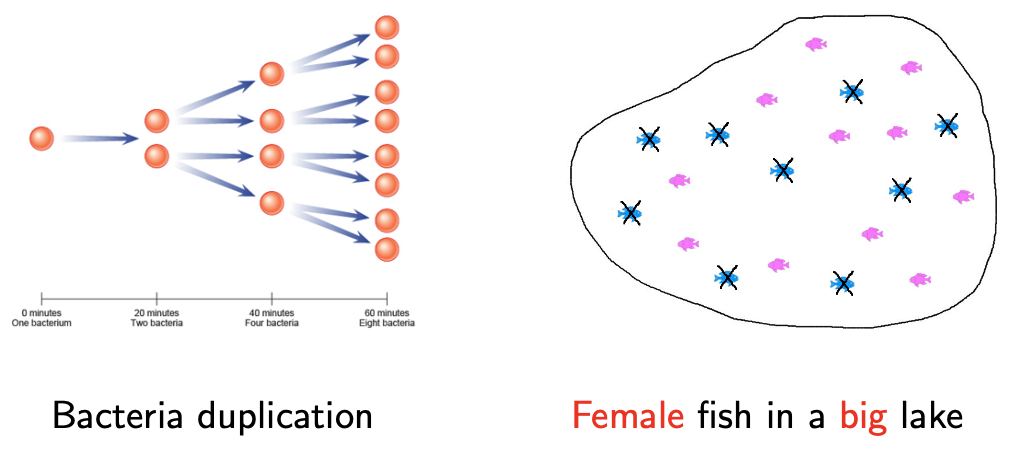
\includegraphics[width=0.8\textwidth]{Images/02-Discrete Dynamical Systems/Example_Linear_Birth_Model.png}
    \caption{Example of populations satisfying the assumption. In the bacteria example in order to assume
            the no children duplication we set $\Delta{t} \leq 20 minutes$} 
\end{figure}

\subsection{Describing the birth process as a relation}
The idea is that the size of the population at time $N(t + \Delta{t})$ will be $\geq$ than $N(t)$ since we assume \textbf{that there is no death occurring in the interval $ [t, t + \Delta{t}$]}. Additionally we know from our assumption that each \textit{adult} individual has $\lambda$ children every $\sigma$ time units.
\par Then, the number of individuals at time $t + \Delta{t}$ corresponds to the number of individuals at time $t$, plus the number of newborns at time $\Delta{t}$:

\begin{center}
    $N(t + \Delta{t}) = N(t) + \lambda{\frac{\Delta{t}}{\sigma}{N(t)}}$
\end{center}
if we group for $N(t)$ then the equation can be rewritten as follows:
\begin{center}
    $N(t + \Delta{t}) = N(t) * (1 + \lambda{\frac{\Delta{t}}{\sigma}}) $
\end{center}
    

\par Where $\frac{\Delta{t}}{\sigma}$ \textbf{describes the birth moments for every \textit{adult} individual in the interval $[t, t + \Delta{t}]$.}

\section{Constructing our algorithm}
Defined our equation \textbf{we can derive a discrete model from it}.
\par We choose a \textbf{time step} (discretization step) that describe an update of the population, in our case \textbf{the time necessary for a newborns to be considered an adult so that it can reproduce}, and we set it as $\Delta{t}$.
\par Instead of representing the equation fully we rewrite it using the \textbf{notation of sequence theory} by instead of using the actual value of the time $\Delta{t}$, we just count the steps. Thus we obtain:
\begin{center}
    $N_{t+1} = r_{d}N_{t}$
\end{center}
where $r$ stands for \textit{rate}; $d$ stands for \textit{discrete}; $r_{d}$ represents the \textbf{constant birth rate} s.t. $r_{d} = \lambda{\frac{\Delta{t}} {\sigma}}$.

\subsection{Defining the general term of our equation}
Given the recurrence relation we can \textit{sometimes} calculate the \textbf{general term}, that is the solution of the recurrence relation. In the case of our linear birth model it is a \textbf{non-recursive definition of $N_{t}$}.
\par To do so we first calculate the first terms of $N_{t}$: $N_{1}, N_{2}, N_{3}, ...$

\begin{center}
    \begin{itemize}[label={}]
        \item $N_{1} = r_{d}N_{0}$

        \item $N_{2} = r_{d}N_{1} = r^{2}_{d}N_{0}$

        \item $N_{3} = r_{d}N_{2} = r^{3}_{d}N_{0}$
    \end{itemize}
\end{center}

We notice how \textit{it seems} that $N_t = r^{t}_{d}N_{0}$, \textbf{but we have to prove it}.
To prove the formula, since we are in the realms of the natural numbers, we can use \textbf{mathematical induction}:

\begin{itemize}[label={}]
    
    \item \textbf{Base Case (t = 0):} $N_{0} = r^{0}_{d}N_{0}$ which is true.
    
    \item \textbf{Induction Case (t = k + 1):} we assume that the formula is correct for $t = 0$ to $t = k$ and check if it is true for $t = k + 1$. We know from assumption that $N_{k+1}$ will be a summation between the previous value for $t = k$ and the newborns in the current step. $N_{k+1} = r_{d}N{k}$ and we know from \textbf{induction hypothesis} that $N_{k} = r^{k}_{d}N_{0}$, thus we can rewrite $N_{k+1}$ as $N_{k+1} = r_{d}(r^{k}_{d}N_{0}) = r^{k+1}_{d}N_{0}$ proving the thesis.  
    
\end{itemize}

Now having the general term $N_{t} = r^{t}_{d}N_{0}$ we can compute the solution of our model.

\subsubsection{Phase portrait}
A way to represent recurrence relations graphically is through \textbf{phase portrait}. It consists in putting in the \textit{Cartesian plane}:
\begin{itemize}
    \item \textbf{x-axis}: $N_{t}$

    \item \textbf{y-axis}: $N_{t+1}$
\end{itemize}

Then in the plane we plot the recurrent relation. First you draw the bisector and you draw the recurrence relation as a function, then by starting from point $(N_{0}, N_{0})$ on the bisector, the other point can be obtained by \textit{"bouncing"} on the curve of the recurrence relation. \textbf{You can see how fast the quantity increases (or decreases) over time}.

\begin{figure}[h]
    \centering
    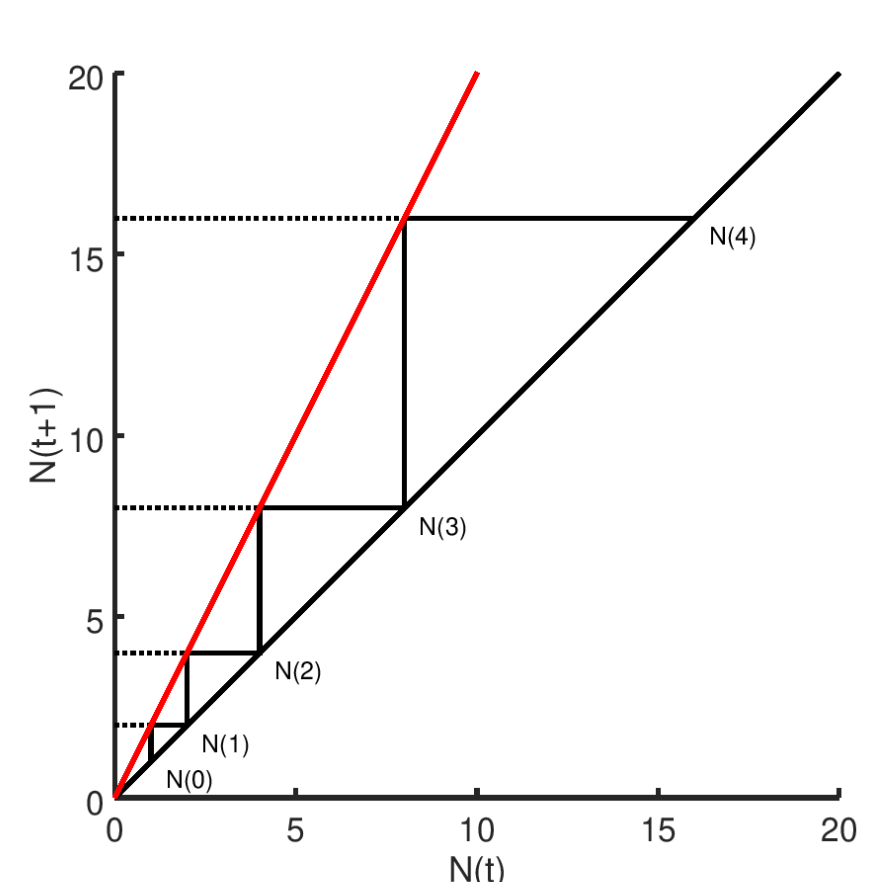
\includegraphics[width=0.5\textwidth]{Images/02-Discrete Dynamical Systems/phase_potrait.png}
    \caption{} 
\end{figure}

\begin{center}
    Above an example of phase portrait in our linear birth model. 
    \par In \textcolor{red}{red} we draw the recurrence equation $N_{t+1} = 2N_{t}$.
    in \textbf{black} the bisector $N_{t+1} = N_{t}$. 
\end{center}

\section{Introducing death in our model}
We complicate our recurrence relation by considering also deaths, so we are adding a negative term that decrease the number of individuals of our population over time. 
\par Assume that, a constant fraction $s_{d}$ \textbf{of adults that die in every time step} $\delta{t}$. Then our recurrence relation now is:
\begin{center}
    $N_{t+1} = r_{d}N_{t} - s_{d}N_{t}$
\end{center}

By grouping for $N_t$ we can rewrite the equation as:

\begin{center}
    $N_{t+1} = (r_{d} - s_{d})N_{t}$
\end{center}

\textbf{Note:} since the number of individuals which die cannot be greater than the whole population, then $ 0 \leq s_{d} \leq 1$

\par Since $r_{d}$ and $s_{d}$ are two constant, one positive and one negative, we can group them together in one single constant $\alpha_{d} = (r_{d} - s_{d})$. We call $\alpha_{d}$ the \textbf{net growth rate}, that is the rate where you discard the individuals who dies. We can rewrite our equations as:

\begin{center}
    $N_{t+1} = \alpha_{d}N_{t}$
\end{center}

The difference in respect of the previous case is that $\alpha_{d}$ will be in general greater than 0, but not necessarily greater than 1.

\subsubsection{General trend of our model}
There could be many possible cases depending on the value of the constant $\alpha_{d}$:

\begin{itemize}

    \item $\alpha_{d} > 1$: the overall behaviour of the population is the same as before, \textbf{since the population at every steps will increase}.

    \item $\alpha_{d} = 1$: the population remains constant, \textbf{since the number of newborns always is equal to the number of dead ones}.

    \item $\alpha_{d} < 1$: if for instance we assume we have less newborns than the death of old individuals, \textbf{then at every step the population reduces}.
    
\end{itemize}

\section{Introducing migration in our model}
Independently from the size of the population, \textbf{we assume a fixed number of individuals arrive in our region}. We only consider people that arrives, so we model the migration using a constant and positive parameter declared as $\beta$. 
\par Then our equation becomes:

\begin{center}
    $N_{t+1} = \alpha_{d}N_{t} + \beta$
\end{center}

with $\beta \geq 0 $ representing the number of individuals entering the population every $\Delta{t}$ time units.

\par By \textbf{mathematical induction} we can prove the general term is:

\begin{center}
    $N_{t} = \alpha^{t}_{d}N_{0} + \sum_{i=0}^{t-1}{a^{i}_{d}\beta}$
\end{center}

where $\sum_{i=0}^{t-1}{a^{i}_{d}\beta}$ accumulates the $\beta$ individuals that arrived in the previous step (from 0 to $t-1$) and the children produced by them at every step.

\subsection{Simulating the migration}
Having our general term, we can see what happens by varying $\alpha_{d}, N_{0}$ and $ \beta:$
\par \textbf{Case $\alpha_{d} > 1$}

\begin{figure}[h]
    \centering
    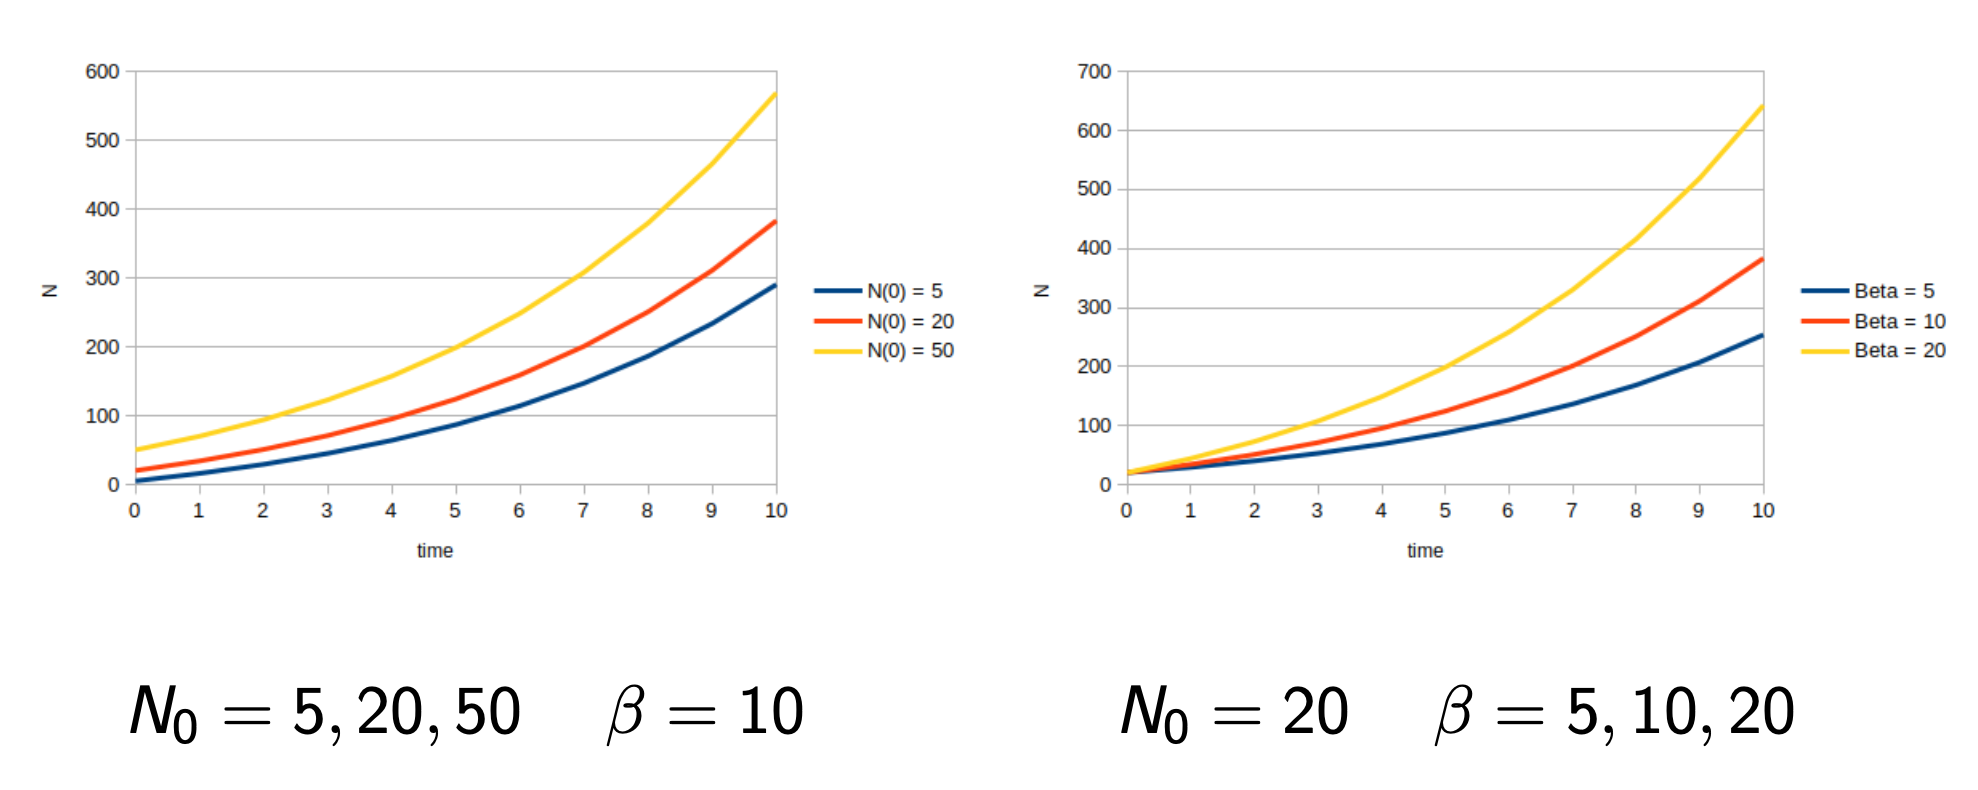
\includegraphics[width=0.9\textwidth]{Images/02-Discrete Dynamical Systems/case_1.png}
    \caption{The dynamics is dominated by the birth process (exponential growth).} 
\end{figure}

\par \textbf{Case $\alpha_{d} = 1$}

\begin{figure}[h]
    \centering
    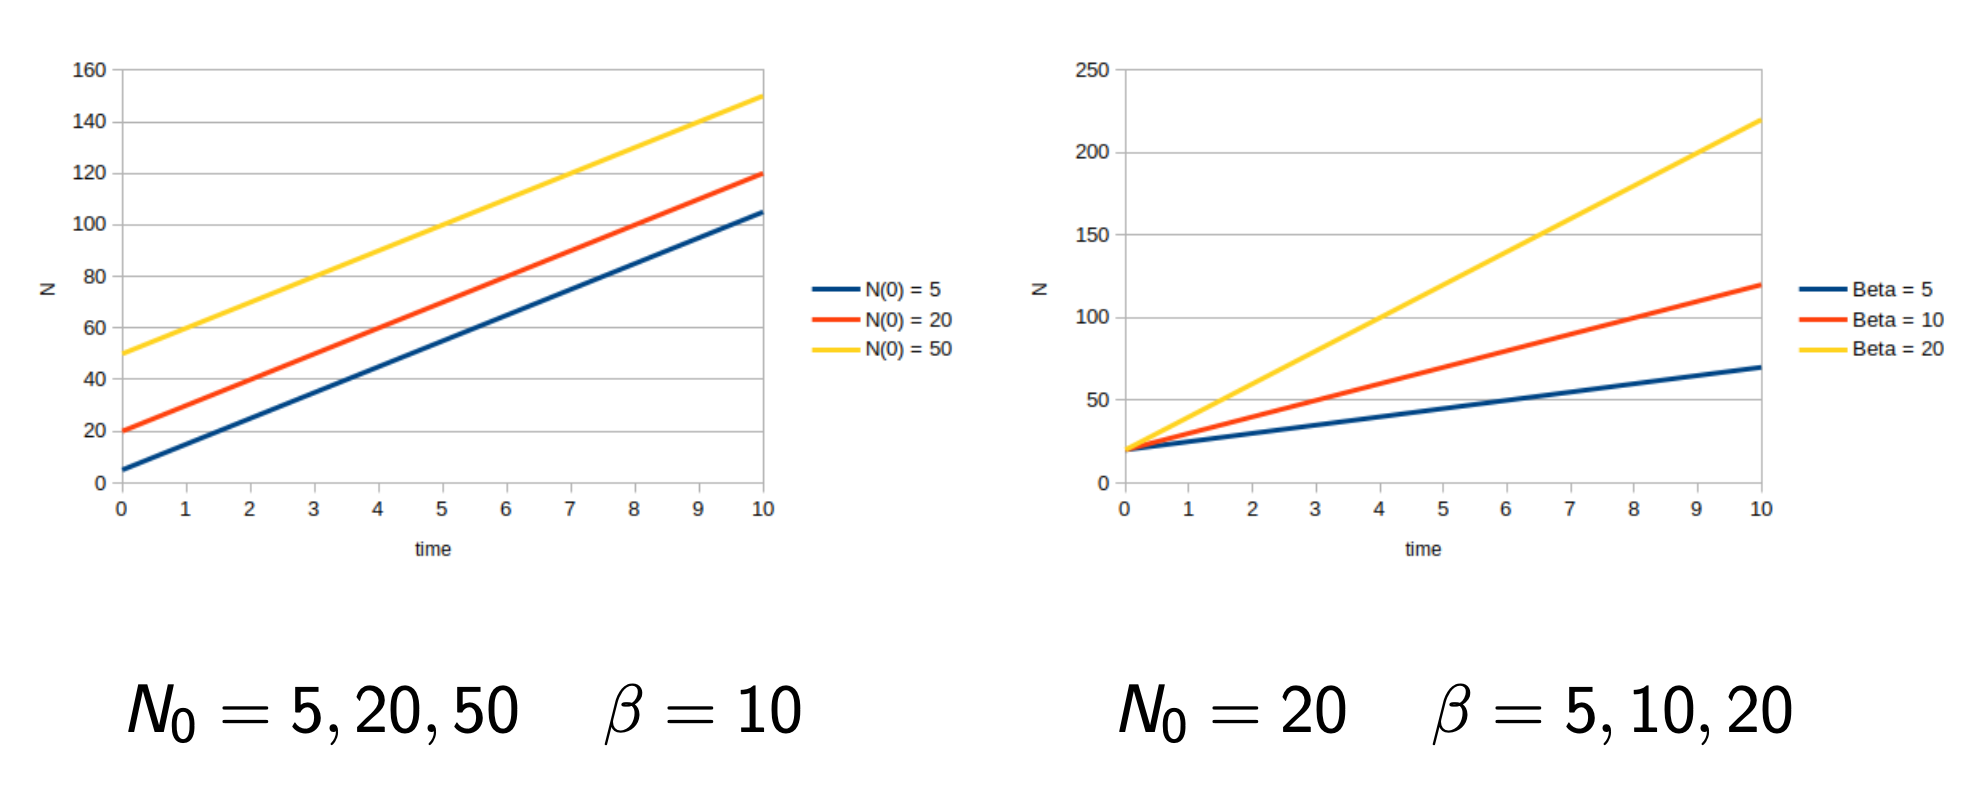
\includegraphics[width=0.9\textwidth]{Images/02-Discrete Dynamical Systems/case_2.png}
    \caption{The dynamics is dominated by the migration process (linear growth).} 
\end{figure}

\par \textbf{Case $\alpha_{d} < 1$}

\begin{figure}[h]
    \centering
    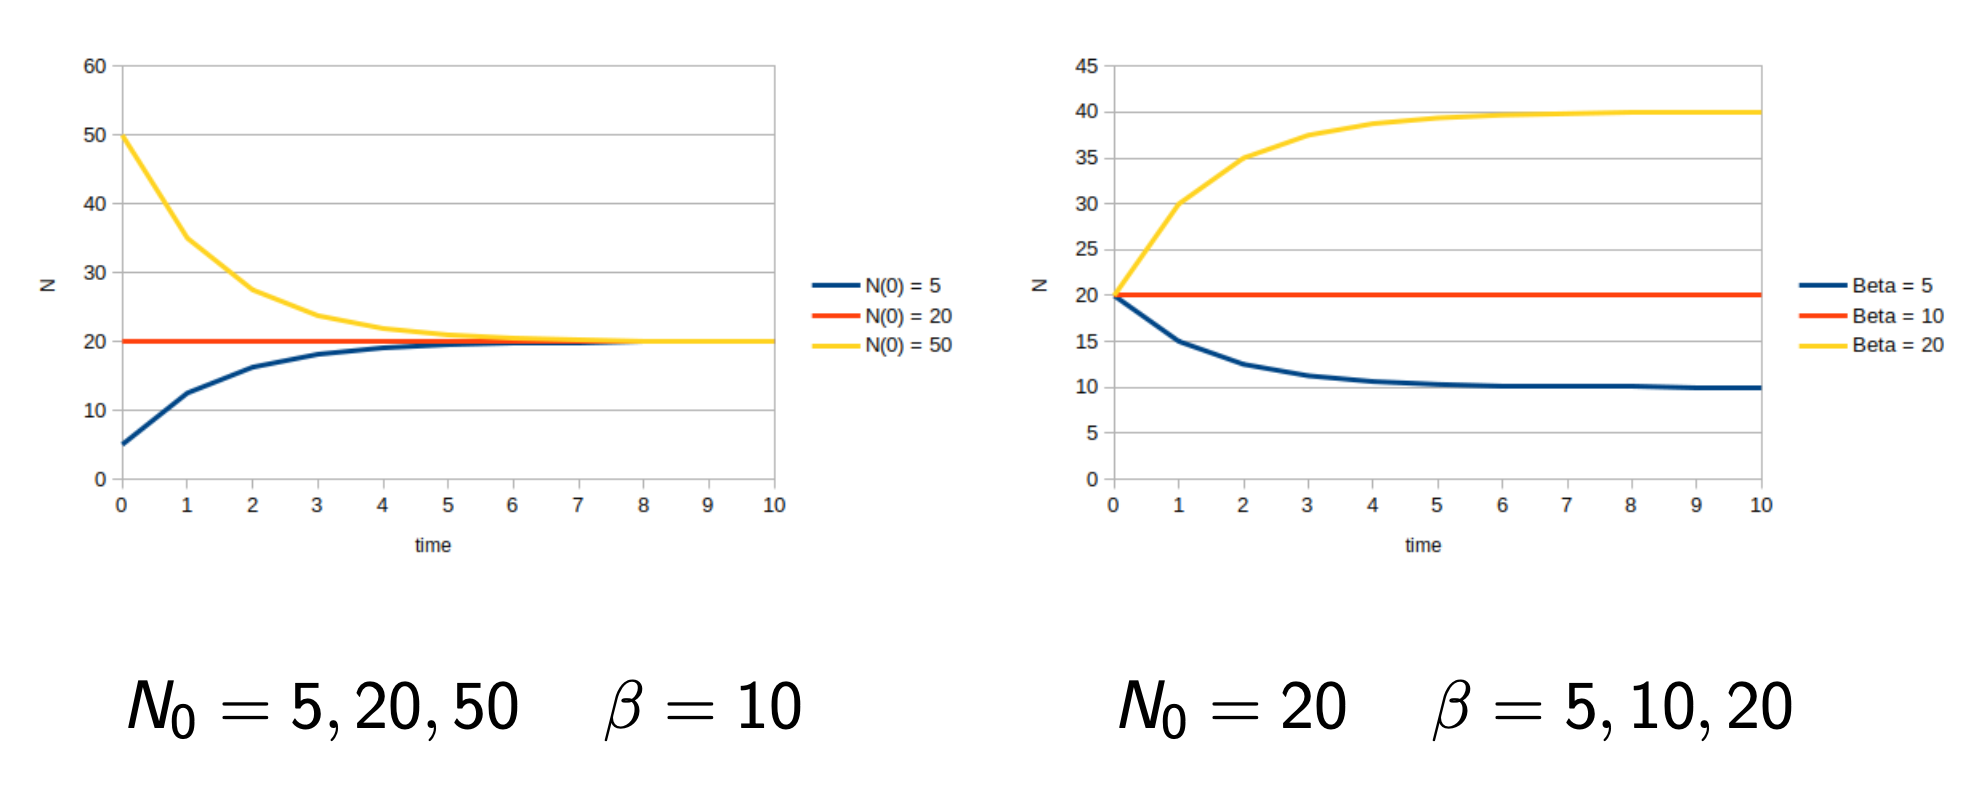
\includegraphics[width=0.9\textwidth]{Images/02-Discrete Dynamical Systems/case_3.png}
    \caption{The population reaches a dynamic equilibrium: a stable state in which opposite phenomena compensate each other (migration compensates deaths). Note that it is independent from $N_{0}$} 
\end{figure}

\subsection{Computing the equilibrium point}
The equilibrium point (also called saturation point) is defined as the moment $t=k+1$ where the computed size of the population is the same as the previous step, that is:

\begin{center}
    $N_{t-1} = N_{t}$
\end{center}

Knowing that $N_{t} = \alpha_{d}N_{t} + \beta$ we solve the equation in regards to $N_{t}$ and obtain:

\begin{center}
    $N_{t} = \frac{\beta}{1 - \alpha_{d}}$
\end{center}

\subsection{Non-linear models}
So far we have described a population where each individual behaves autonomously, which do not fit the definition of complex system (many components with very simple individual behaviour \textbf{that interact with each other and the environment}). Introducing interaction between the individuals \textbf{requires a non-linear model} (previously we used a linear one). In our (Non-linear) Birth Model now the environment has limited resources such as food and place, thus requiring that the individuals compete \textbf{(a form in interaction)} for survival.

\section{Rewriting our equation}
For simplicity assume we are in a closed environment (no migration), then we define $K$ as the \textbf{carrying capacity of the environment}, meaning that in the environment there is enough food and space for $K$ individuals.
\par The population is still governed by the birth rate, but now death is no more a constant, instead is negatively influenced by $K$:

\begin{center}
    $N_{t+1} = r_{d}N_{t}(1 - \frac{N_{t}}{K})$
\end{center}
\textbf{Note:} this non-linear equation is called \textbf{logistic equation} (it is an alternative formulation)

So now the birth rate is modulated by the ratio of occupancy on the environment $\frac{N_{t}}{K}$:

\begin{itemize}

    \item $N_{t}$ close to 0 : we have a simple birth process with rate $r_{d}$ (exponential growth). 

    \item $N_{t}$ increases: the growth tends to stop.

\end{itemize}

Eventually the population reaches a \textbf{dynamic equilibrium} representing the situation in which environment resources are fully exploited (\textbf{saturation})

\begin{figure}[h]
    \centering
    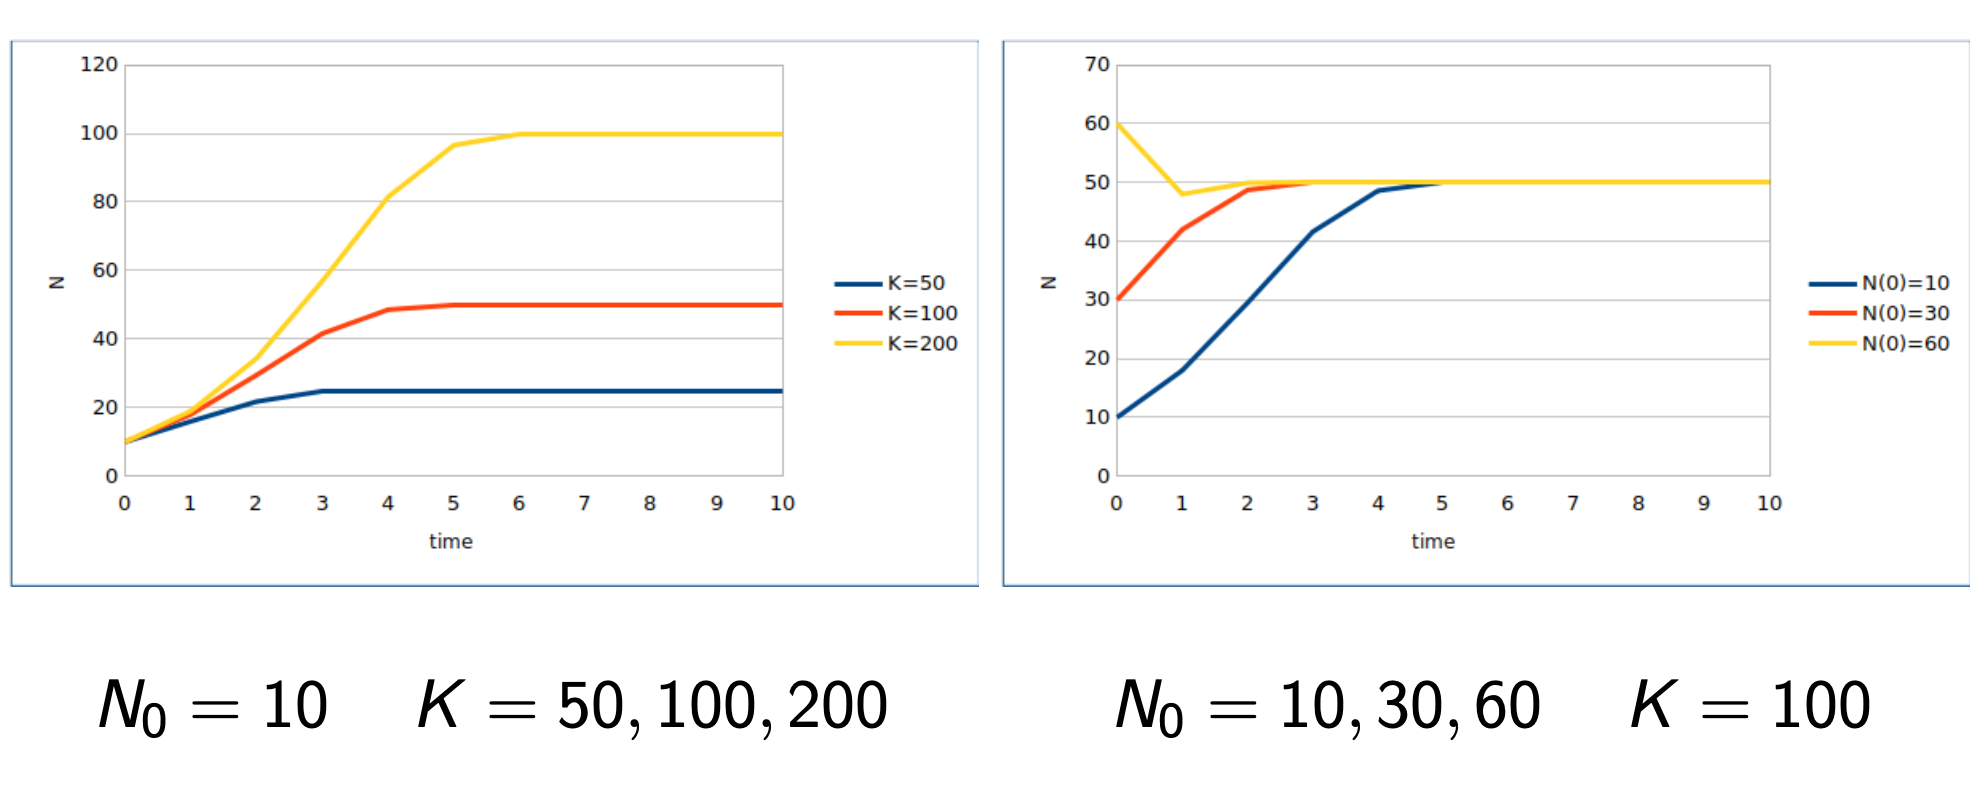
\includegraphics[width=0.9\textwidth]{Images/02-Discrete Dynamical Systems/Non-linear .png}
    \caption{The first graph shows a case where the equilibrium point depends on $K$. The second graph shows me that the equilibrium point is independent from the initial number of individuals.} 
\end{figure}

\section{Removing homogeneity}
For now we have considered an homogeneous population, but in realistic case we have different individuals with different features and we want to consider each group of individuals. In the system point of view this requires not just a single recurrence equation, but a \textbf{system of recurrence equations}. 
\par consider a population of fishes that live in a pond. Each individual can either be a male fish, modelled as $M_t$ or a female fish, modelled as $F_t$. We consider that a small part of males dies because of fights among them (death rate $s_d$).
\par then we construct a system of recurrence equations:


\[
\begin{cases} 
        F_{t+1} = r_{d}F_{t}(1 - \frac{F_{t} + M_{t}} {K}) \\
        M_{t+1} = r_{d}F_{t}(1 - \frac{F_{t} + M_{t}}{K}) - s_{d}M_{t}\\
\end{cases}
\]

where:
\begin{itemize}
    \item $r_{d}F_{t}$ represent the number of child born, note that they are generated by females.

    \item $F_{t} + M_{t}$ describes the whole population size (to be related with the carrying capacity K).
\end{itemize}

\section{Limitation of discrete dynamical models}
Discretization of the system dynamics may introduce inaccuracies: recurrence equations assume that nothing happens during the $\Delta{t}$ time that occurs between $N_{t}$ and $N_{t+1}$. Adjusting $\Delta{t}$ to be smaller usually correspond to more accurate approximations, more precisely we should let $\Delta{t}$ tend to 0.

